\subsection{Introduction}
Machine Learning (ML) is the set of practices that allow to obtain a prediction model from a set of input/output (dataset), in a process called training. 
Dataset is a collection of entries with a number of fields (features) that describe the data.
The dataset is often divided in two pieces: training dataset and validation dataset.

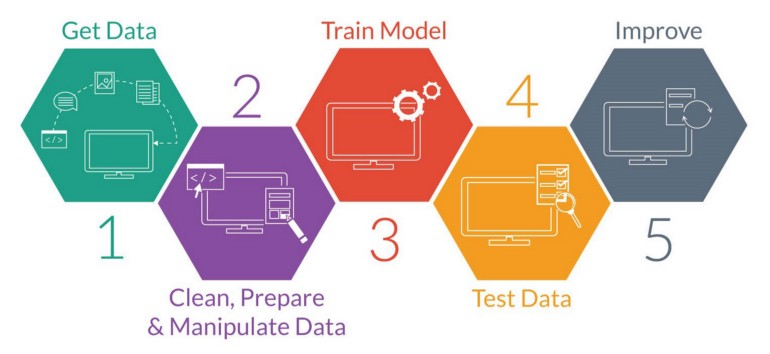
\includegraphics[scale=0.3]{pictures/machine_learning_process.jpeg}

\subsubsection{Steps}
\begin{enumerate}
    \item Formulating the problem
    \item Framing the problem: identify which type of ML approaches (one or more) fits best the problem
    \item Design the dataset
    \item Training
    \item Validating the model
\end{enumerate}



\subsubsection{Problem Framing}

\begin{itemize}
    \item Supervised Learning: if data are labeled, so the output is a feature of the dataset; the goal is finding the relation between the features and the labels.
        \begin{itemize}
            \item Classification: pick one of the N labels (binary, multi-class)
                \begin{itemize}
                    \item Logistic Regression
                    \item SVM (Support Vector Machine)
                    \item ANN
                    \item Decision Trees
                    \item Random Forest
                \end{itemize}
            \item Regression: predict numerical values
                \begin{itemize}
                    \item Linear Regression
                    \item Polynomial Regression
                \end{itemize}
            \item Deep Learning:
                \begin{itemize}
                    \item CNN
                    \item RNN
                \end{itemize}
        \end{itemize}
    \item Unsupervised Learning: if data are not labeled, so the output is not in the dataset; the goal is to identify meaningful patterns in the data and build its own labels (clusters).
        \begin{itemize}
            \item Clustering: group similar data (K-Means, SVD, PCA)
            \item Association: infer likely association patterns in data
            \item Dimensionality Reduction
            \item Anomaly Detection
        \end{itemize}
    \item Reinforcement Learning: the model (agent) is set up and receives reward (reward function) when it performs the specified task.
        \begin{itemize}
            \item Dynamic Programming
            \item Monte Carlo methods
        \end{itemize}
\end{itemize}



\subsubsection{Overfiting/Underfitting}
Overfitting occurs when features are too much and the model obtained track very well the training data, which can be affected by noise, but does not pass validation.
Underfitting occurs when features are not enough to fit a proper model, then is poor both in traingn and in validation.





\subsection{Validation}


